% This file was created by tikzplotlib v0.9.1.
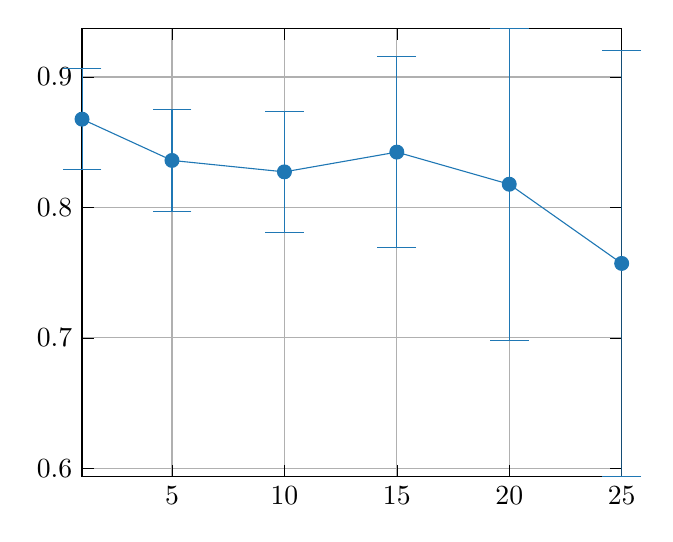
\begin{tikzpicture}

\definecolor{color0}{rgb}{0.12156862745098,0.466666666666667,0.705882352941177}

\begin{axis}[
tick pos=both,
x grid style={white!69.0196078431373!black},
xmajorgrids,
xmin=1, xmax=25,
xtick style={color=black},
y grid style={white!69.0196078431373!black},
ymajorgrids,
ymin=0.593704093157292, ymax=0.937353539412938,
ytick style={color=black}
]
\path [draw=color0]
(axis cs:1,0.829137660288607)
--(axis cs:1,0.906164642130413);

\path [draw=color0]
(axis cs:5,0.796868799247784)
--(axis cs:5,0.87515420914943);

\path [draw=color0]
(axis cs:10,0.781033771932043)
--(axis cs:10,0.873460326673177);

\path [draw=color0]
(axis cs:15,0.768977364979775)
--(axis cs:15,0.915824752463575);

\path [draw=color0]
(axis cs:20,0.698202003721037)
--(axis cs:20,0.937353539412938);

\path [draw=color0]
(axis cs:25,0.593704093157292)
--(axis cs:25,0.920422658093218);

\addplot [color0, mark=-, mark size=7, mark options={solid}, only marks]
table {%
1 0.829137660288607
5 0.796868799247784
10 0.781033771932043
15 0.768977364979775
20 0.698202003721037
25 0.593704093157292
};
\addplot [color0, mark=-, mark size=7, mark options={solid}, only marks]
table {%
1 0.906164642130413
5 0.87515420914943
10 0.873460326673177
15 0.915824752463575
20 0.937353539412938
25 0.920422658093218
};
\addplot [color0, mark=*, mark size=2.5, mark options={solid}]
table {%
1 0.86765115120951
5 0.836011504198607
10 0.82724704930261
15 0.842401058721675
20 0.817777771566987
25 0.757063375625255
};
\end{axis}

\end{tikzpicture}
